\section{Results \& Discussion}\label{sec:results}

\subsection{Fitting Sorption Parameters}\label{sec:results_sorption_fit}

Using the numerical fitting scheme described in section \ref{sec:indoor_environment} with the sorption data from the method described in section \ref{sec:experimental_method}, the kinetic sorption parameters $k_1$ and $k_2$ are fitted.
Figure \ref{fig:sorption_fit} shows the result of this fitting and the sorption data for three select materials - wood, Appling soil, and cinderblock concrete.
The $k_1$ and $k_2$ represent the rate at which TCE desorbs and sorbs respectively onto/from the material of interest.
The equilibrium sorption constant is, using the formulation in \eqref{eq:sorption_rate}, given by
\begin{equation}
  K = \frac{k_1}{k_2}
\end{equation}
and is used as the sorption isotherm.
Here a small $K$ indicate that there is a greater propensity for contaminant sorption.\par

To use the soil sorption isotherm in \eqref{eq:mass_transport} $K$ needs to be converted from being unitless to $\mathrm{m^3/kg}$.
This is done by multiplying the inverse of $K$ isotherm with inverse of the soil bulk density $\rho_b$, which is taken to be $1460 \; \mathrm{kg/m^3}$.
\begin{equation}
  K_\mathrm{ads} = \frac{1}{K \rho_b} = 5.28 \; \mathrm{(m^3/kg)}
\end{equation}

\begin{figure}[htb!]
  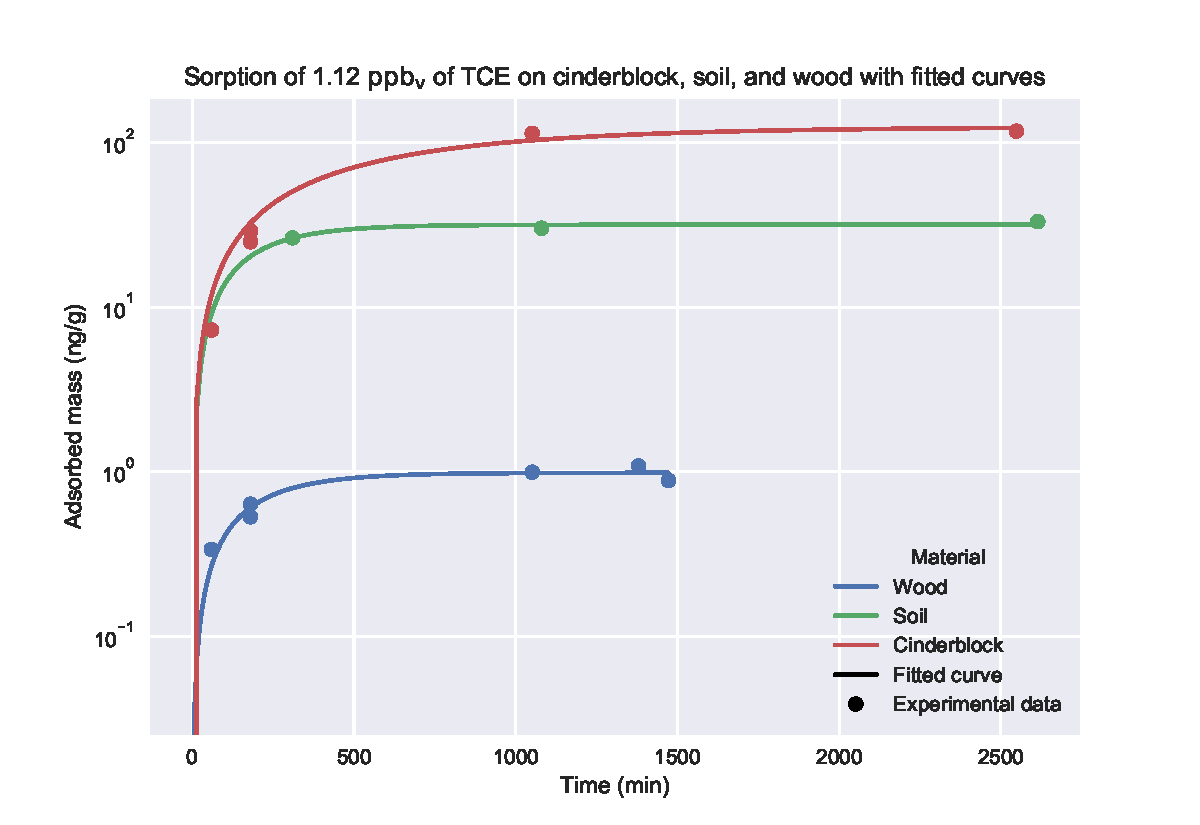
\includegraphics[width=\textwidth]{sorption_fit.pdf}
  \caption{Experimental data of sorption of TCE onto three select materials as well as fitted sorption rates based on the kinetic model \eqref{eq:sorption_rate}.}
  \label{fig:sorption_fit}
\end{figure}

% TODO: Shuai: Some thoughts or comments about these values? I.e. why is cinderblock so much larger?
Table \ref{tbl:sorption_fit} shows the fitted parameters for the tested materials.
Based on this these results we can see that cinderblock and soil have orders of magnitude larger sorption capacities than wood or drywall does.
We can also see by the $k_2$ values that soil and cinderblock sorb quickly, much faster than a material with similar sorptive capacity such as paper.
% Lots of "why is this?" here...

\begin{table}[htb!]
  \caption{Fitted kinetic sorption parameters based on sorption experiment data.}
  \label{tbl:sorption_fit}
  \centering
  \begin{tabular}{l c c c}
    \toprule
    Material & $k_1 \; \mathrm{(1/hr)}$ & $k_2 \; \mathrm{(1/hr)}$ & $K$ \\
    \hline
    Wood & 0.32 & 44.90 & $7.10 \cdot 10^{-3}$ \\
    Drywall & 0.41 & 87.94 & $4.65 \cdot 10^{-3}$ \\
    Carpet & 0.26 & 58.74 & $4.42 \cdot 10^{-3}$ \\
    Paper & 0.04 & 88.37 & $4.55 \cdot 10^{-4}$ \\
    Soil & 0.34 & 2636.57 & $1.30 \cdot 10^{-4}$ \\
    Cinderblock & 0.10 & 4175.16 & $2.40 \cdot 10^{-5}$ \\
    \bottomrule
  \end{tabular}
\end{table}



\subsection{Soil Sorption's Retarding Effect}\label{sec:retardation_effect}

Building pressurization is a key factor in VI that influences the advective contaminant transport.
The magnitude of change in response to a pressurization change is significantly influenced by a range of factors, such as soil permeability, foundation depth, or soil moisture.
To demonstrate the effect that soil sorption has on contaminant soil mass transport in the VI context, we run two types transient simulation where initially the modeled structure is at a steady -5 Pa, i.e. slightly depressurized.
At the start of the simulation, the building building is 1) further depressurized to -15 Pa, or 2) overpressurized to 15 Pa, and the simulation is allowed to run for 72 hours.
\begin{align}
  \text{Depressurization}: \; \Delta p_\mathrm{in/out} &= \begin{cases}
    -5, \; &t = 0 \; \mathrm{(hr)} \\
    -15, \; &0 < t \leq 72 \; \mathrm{(hr)}
\end{cases}\label{eq:equilibrium_depressurization}\\
\text{Overpressurzation}: \; \Delta p_\mathrm{in/out} &= \begin{cases}
  -5, \; &t = 0 \; \mathrm{(hr)} \\
  15, \; &0 < t \leq 72 \; \mathrm{(hr)}
\end{cases}\label{eq:equilibrium_overpressurization}
\end{align}
For each of these cases, the simulation is run using two different soil types - sand and sandy loam.
Sand is assumed here to not sorb any TCE, while for sandy loam a range of sorption isotherms are used.
These range from no sorption ($K_\mathrm{ads} = 0 \; \mathrm{(m^3/kg)}$) to the experimentally determined sorption isotherm ($K_\mathrm{ads} = 5.28 \; \mathrm{(m^3/kg)}$) in intervals multiplicative by $10^{-2}$. With the experimentally determined isotherm, we see that the ratio between sorbed concentration and soil-gas phase concentration is 7708, i.e. there is a much larger amount of sorbed contaminant.
When $K_\mathrm{ads} = 5.28 \cdot 10^{-4} \; \mathrm{(m^3/kg)}$ this ratio is roughly unity (0.77), which is good to keep in mind in the following discussion. % TODO: Make sure you change this value if you rerun the simulation later with a different H
These ranges of values can be used both to represent a soil that has a smaller sorptive capacity or a situation where the sorbed and gas phase has not quite reached equilibrium.\par

\begin{figure}[!htb]
  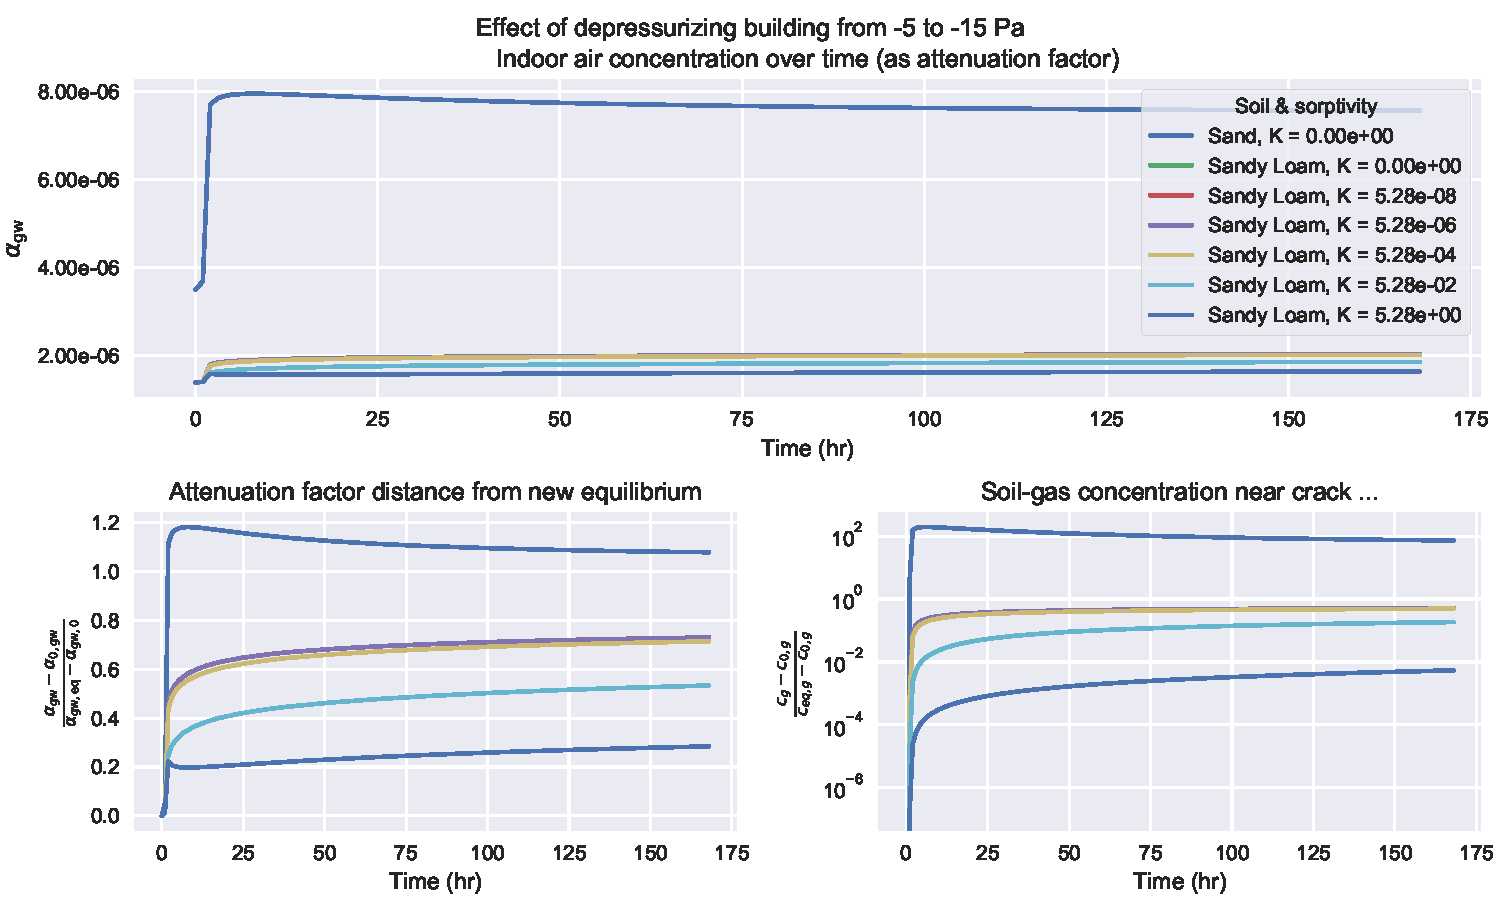
\includegraphics[width=\textwidth]{equilibrium_retardation_depressurization.pdf}
  \caption{}
  \label{fig:equilibrium_depressurization}
\end{figure}

In the top panel of Figure \ref{fig:equilibrium_depressurization}, the indoor air contaminant concentration as the simulated building is undergoing the pressurization in \eqref{eq:equilibrium_depressurization} case.
Here we can see that for the case when the surrounding soil consists of sand, the indoor concentration increases rapidly as the building is further pressurized.
The rate of increase decreases significantly for the sandy loam cases, and progressively retards are the sorbed mass increases ($K_\mathrm{ads}$ increases).\par

The bottom left panel shows how far away the indoor air concentration (as attentuation factor) for each case is from reaching equilibrium.
At the start of the simulation, the building starts with an attenuation of $\alpha_0$, which is the steady-state concentration when the building is pressurized with -5 Pa.
As the building is further depressurized to -15 Pa, the indoor air concentration will approach a new equilibrium state $\alpha_{eq}$ (the result of which is from a steady-state simulation at that pressurization).
By plotting $\frac{|\alpha-\alpha_0|}{|\alpha_{eq}-\alpha_0|}$ we can easily see how far away we are from the new equilibrium state, and a value of 0 represents that we are at the initial concentration, i.e. $\alpha = \alpha_0$, and a value of 1 represents $\alpha = \alpha_{eq}$.\par

This sort of analysis is applied to the bottom right panel as well, but instead of the indoor air concentration (as attentuation factor), we consider the average soil-gas concentration in a 5 cm diameter cylinder that envelop the entire perimeter crack.
The choice of 5 cm is arbitrary, but helps illustrate what happens with the near-foundation-crack soil-gas concentration, changes in which allow us to better understand how the contaminant is transported into the building from the soil.
The same could be done for the soil-gas velocity of course, but the rate of soil-gas velocity change is virtually the same for all of these cases, and reaches the new equilibrium velocity very quickly (much faster than the concentration) and is thus omitted from the figure.\par

Before discussing the role of sorption here, we can first compare the non-sorbing sand and sandy loam cases.
Due to the higher permeability and lower moisture content, sand is significantly more permeable to gas flow than sandy loam (see Table \ref{tbl:model} for permeability values).
Consequently the advective transport through the foundation crack is much more significant, which is indicated by a Péclet number of around 4 versus 0.2 at a -15 Pa pressurization for sand and sandy loam respectively.\par

Due to the advection dominated transport mechanism in the sand case, the indoor air concentrations are temporarily elevated above the equilibrium concentration at -15 Pa, while the soil-gas concentration moves further away from equilibrium.
(Note that the absolute distance from equilibrium is plotted in Figure \ref{fig:equilibrium_depressurization} which is why at first glance one might think that the soil-gas concentration is two order of magnitude higher initially, but actually is two order of magnitude lower.)
This phenomena occurs because initially more contaminants are drawn into the building from the near crack area than can be resupplied, temporarily depleting the local soil-gas contaminant concentration.\par

One can notice that many of the sandy loam lines overlap, and start diverging from each other when $K_\mathrm{ads} = 5.28 \cdot 10^{-4} \; \mathrm{(m^3/kg)}$, at the point where the ratio of sorbed and soil-gas concentration are roughly equal.
We see that this divergence occurs simultaneously in the indoor air and soil-gas contaminant concentration.
However, since the indoor air concentration depend on the soil-gas concentration, we know that this is where the relevant difference is.\par

The simple reason for this is that it is at this threshold the sorptive contribution to the retardation factor \eqref{eq:retardation_factor} starts to becomes larger than the other terms.
\begin{equation}
   \rho_b K_H K_\mathrm{ads} > \theta_w + \theta_g K_H
\end{equation}
Thus it is at this point that the contaminant transport in the soil starts to become retarded by sorption.
The physical reason for this is that the partitioning between the various phases gives a residence time as the contaminant is transported.
Under VI conditions, the values of $\theta_w + \theta_g K_H$ are bounded to relatively small values, while $K_\mathrm{ads}$ can vary by orders of magnitude, making sorption potentially a very significant retarder for soil transport.\par

Figure \ref{fig:equilibrium_overpressurization} shows the same sort of analysis as in Figure \ref{fig:equilibrium_depressurization} but with the building pressurization following \eqref{eq:equilibrium_overpressurization}.
The results here are more or less the same, with the notable exception that in the sand case, the final equilibrium concentration is not initially exceeded.
As the building is overpressurized, the indoor contaminant are pushed out into the soil.
Since the indoor air concentration is lower than the soil-gas concentration, this is entirely expected.\par

\begin{figure}[!htb]
  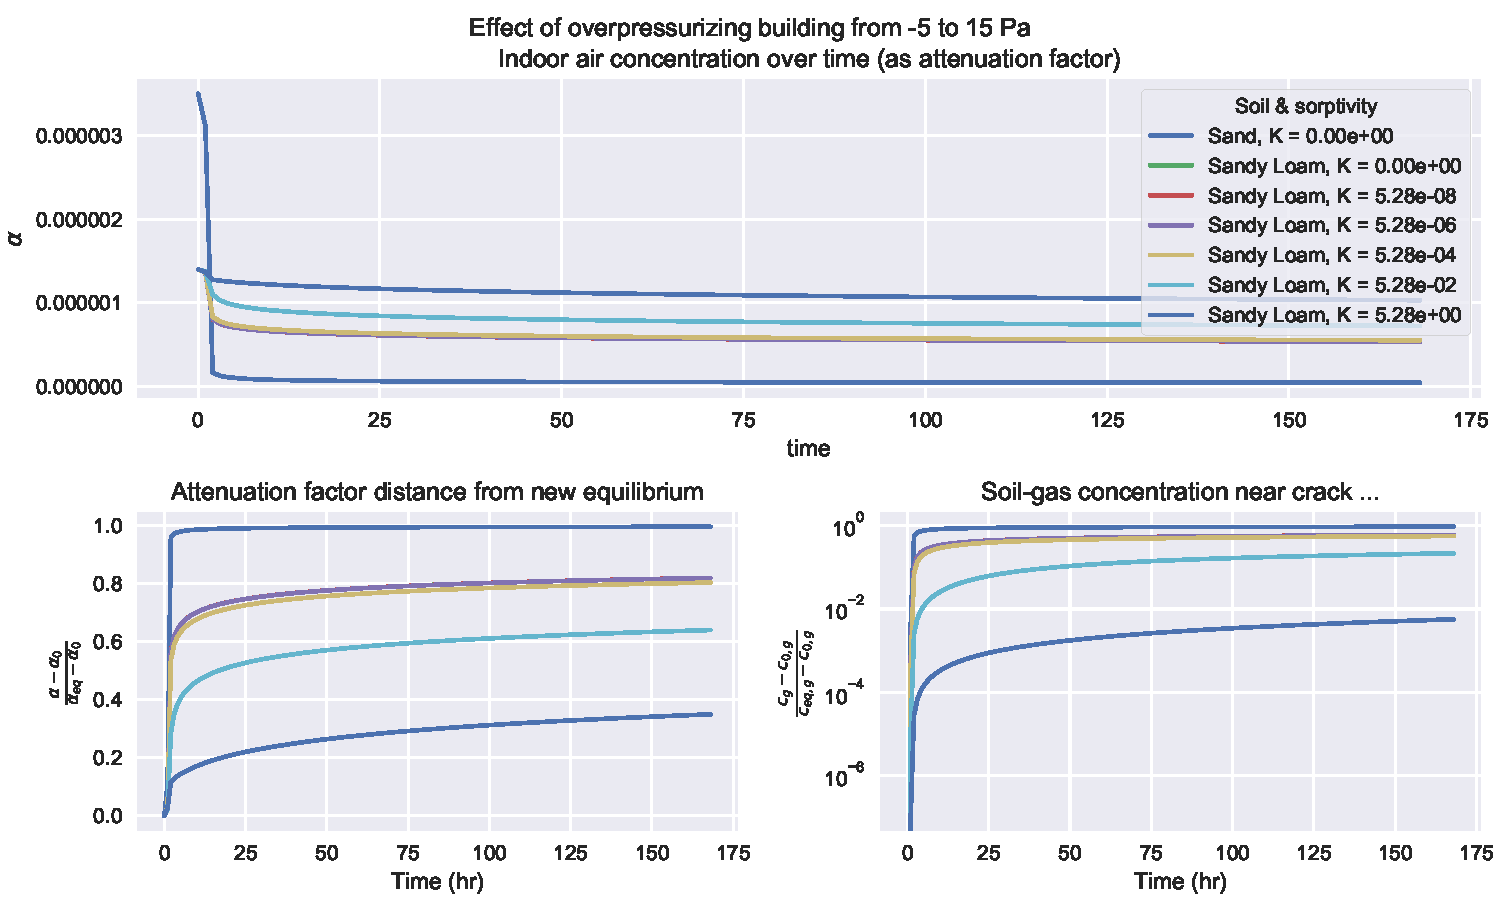
\includegraphics[width=\textwidth]{equilibrium_retardation_overpressurization.pdf}
  \caption{}
  \label{fig:equilibrium_overpressurization}
\end{figure}

% TODO: Some concluding remarks or keep this solely for the conclusion section?

\subsection{Indoor Material Sorption And Dynamics}\label{sec:results_indoor_sorption}

We have now explored the effect that sorption has on contaminant mass transport in the sub-surface soil and seen its retarding effect.
Now we turn to exploring the effect of sorption onto/from various indoor materials has on the indoor air contaminant concentration.
(Here we assume that there is no soil sorption.)\par

To study this we consider the basement (the indoor air space) and assume that the inside surfaces are entirely made up of one of the materials we studied in \ref{sec:results_sorption_fit}.
We also assume that the material covering the indoor surfaces has a certain thickness or depth that the contaminants can penetrate - giving a certain volume or mass of sorbing material in the indoor.
Table \ref{tbl:sorbed_material} shows the surface area, penetration depth, and volume of each material studied.
While obviously some of these rooms are non-conventional and arbitrarily designed, i.e. you're unlikely to find a room with carpeted walls, floors, and ceiling, they do present some limiting cases of the potential effect of sorption onto/from these materials.\par

% TODO: Do I want to include some more information/data here? Sorbed mass at t0?
\begin{table}[htb!]
  \centering
  \begin{tabular}{l c c}
    \toprule
    Material & $d_\mathrm{p} \; \mathrm{(mm)}$ & $V_\mathrm{mat} \; \mathrm{(m^3)}$ \\
    \hline
    Cinderblock & 5 & 1.6 \\
    Wood & 1 & 0.32 \\
    Drywall & 10 & 3.2 \\
    Carpet & 10 & 3.2 \\
    Paper & 0.1 & 0.032 \\
    \bottomrule
  \end{tabular}
  \caption{The assumed contaminant penetration depth and subsequent volume of the sorbing indoor materials. The material surface area is assumed to be the same, and each material completely cover the surfaces of a 10x10x3 meter room.}
  \label{tbl:sorbed_material}
\end{table}

The modeled building then undergoes a pressurization cycle, where at start of the simulation it is depressurized at -5 Pa and at steady-state.
The building is then sequentially depressurized to -15 Pa, then pressurized to 15 Pa, and finally again depressurized to -5 Pa.
For each sequence, the new pressurization is maintained for 24 hours.
This pressurization cycle may be seen in the top left panel of \ref{fig:indoor_sorption_cycle}.
The choice of pressurization cycle is somewhat arbitrary, but ours can be used to represent limiting cases of natural pressurization variation, or artificially induced pressurization.
Figure \ref{fig:indoor_sorption_cycle} shows the result of these simulations.\par

First we consider the reference case - where there is no sorbing indoor materials present.
(The blue line is the reference case, which may be difficult to see as the wood and )
Here we see that as the building is depressurized, the indoor air contaminant concentration increases quickly in response to the pressurization change.

\begin{figure}[!htb]
  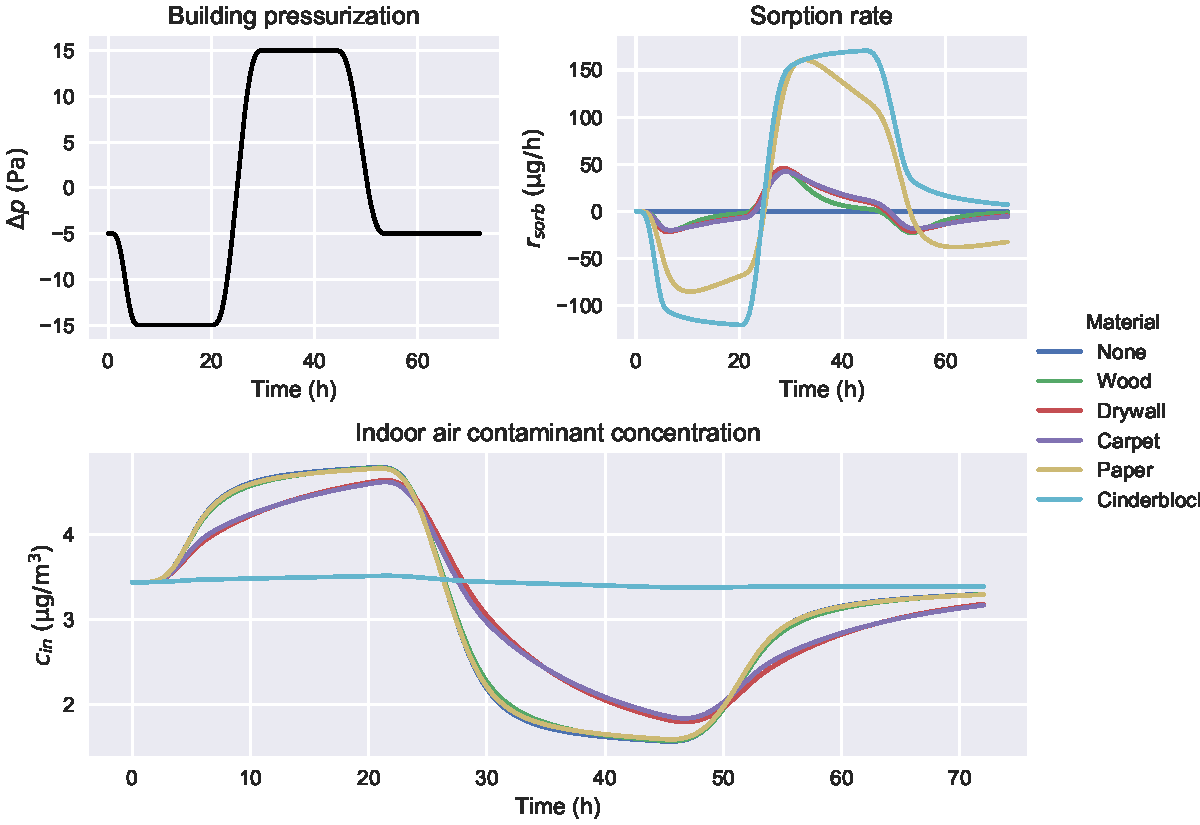
\includegraphics[width=\textwidth]{sorption_indoor_cycle.pdf}
  \caption{
  Comparison of how sorption onto/from various indoor materials affect the indoor air contaminant concentration (bottom) of a building that undergoes a pressurization cycle (top left). The rate of de- and sorption for each considered material during the cycle are also shown (top right) and is governed by \eqref{eq:sorption_rate}.}
  \label{fig:indoor_sorption_cycle}
\end{figure}



\subsection{Indoor Material Sorption And Mitigation}\label{sec:results_indoor_mitigation}


\begin{figure}[!htb]
  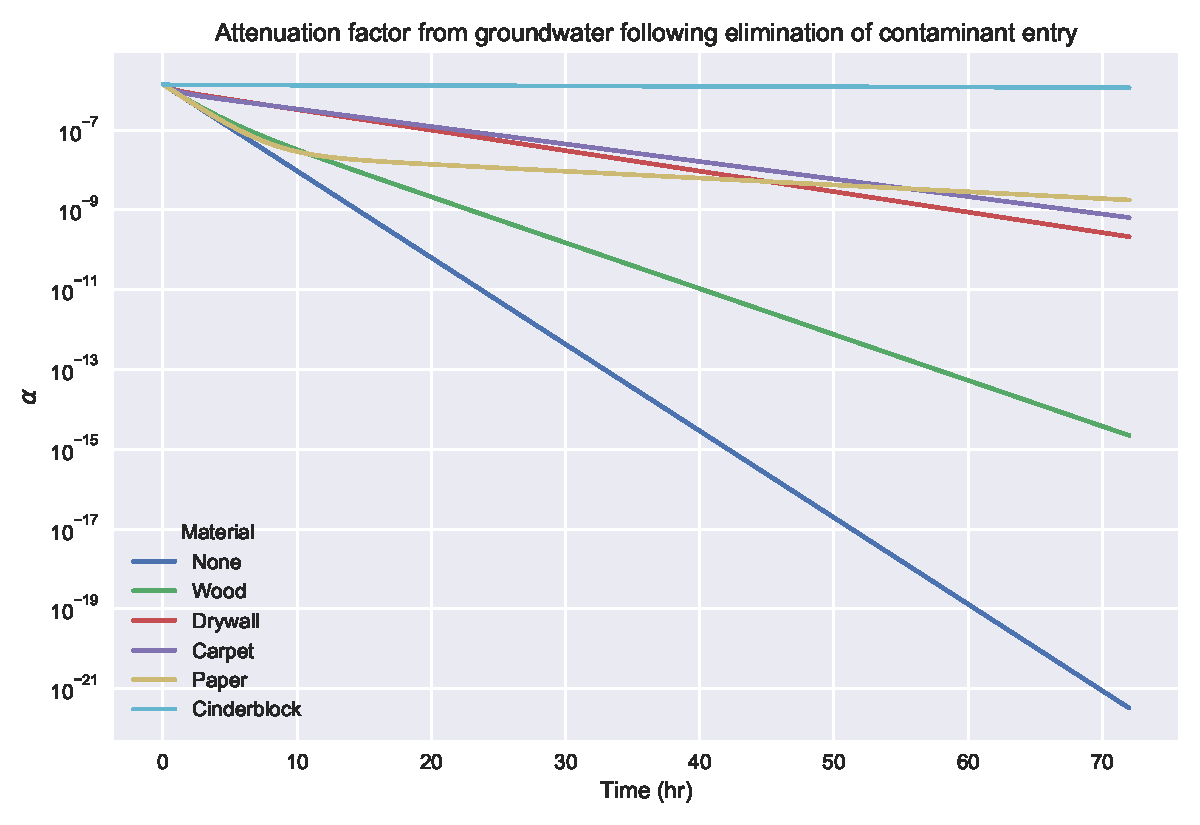
\includegraphics[width=\textwidth]{sorption_mitigation.pdf}
  \caption{}
  \label{fig:sorption_mitigation}
\end{figure}
